\section*{Anexo I: Ejemplo del procesamiento digital de ondas}
\addcontentsline{toc}{section}{Anexo I: Ejemplo del procesamiento digital de ondas}
\vspace{3\baselineskip}

A continuación se ilustra de manera secuencial, el procesamiento digital del impulso mediante el motor de cálculo, desarrollado a partir de la norma IEC 60060~\cite{iec60060}, que se explicó en la sección \ref{subsec:motor_calculo}.

\vspace{3\baselineskip}
\begin{figure}[H]
    \centering
    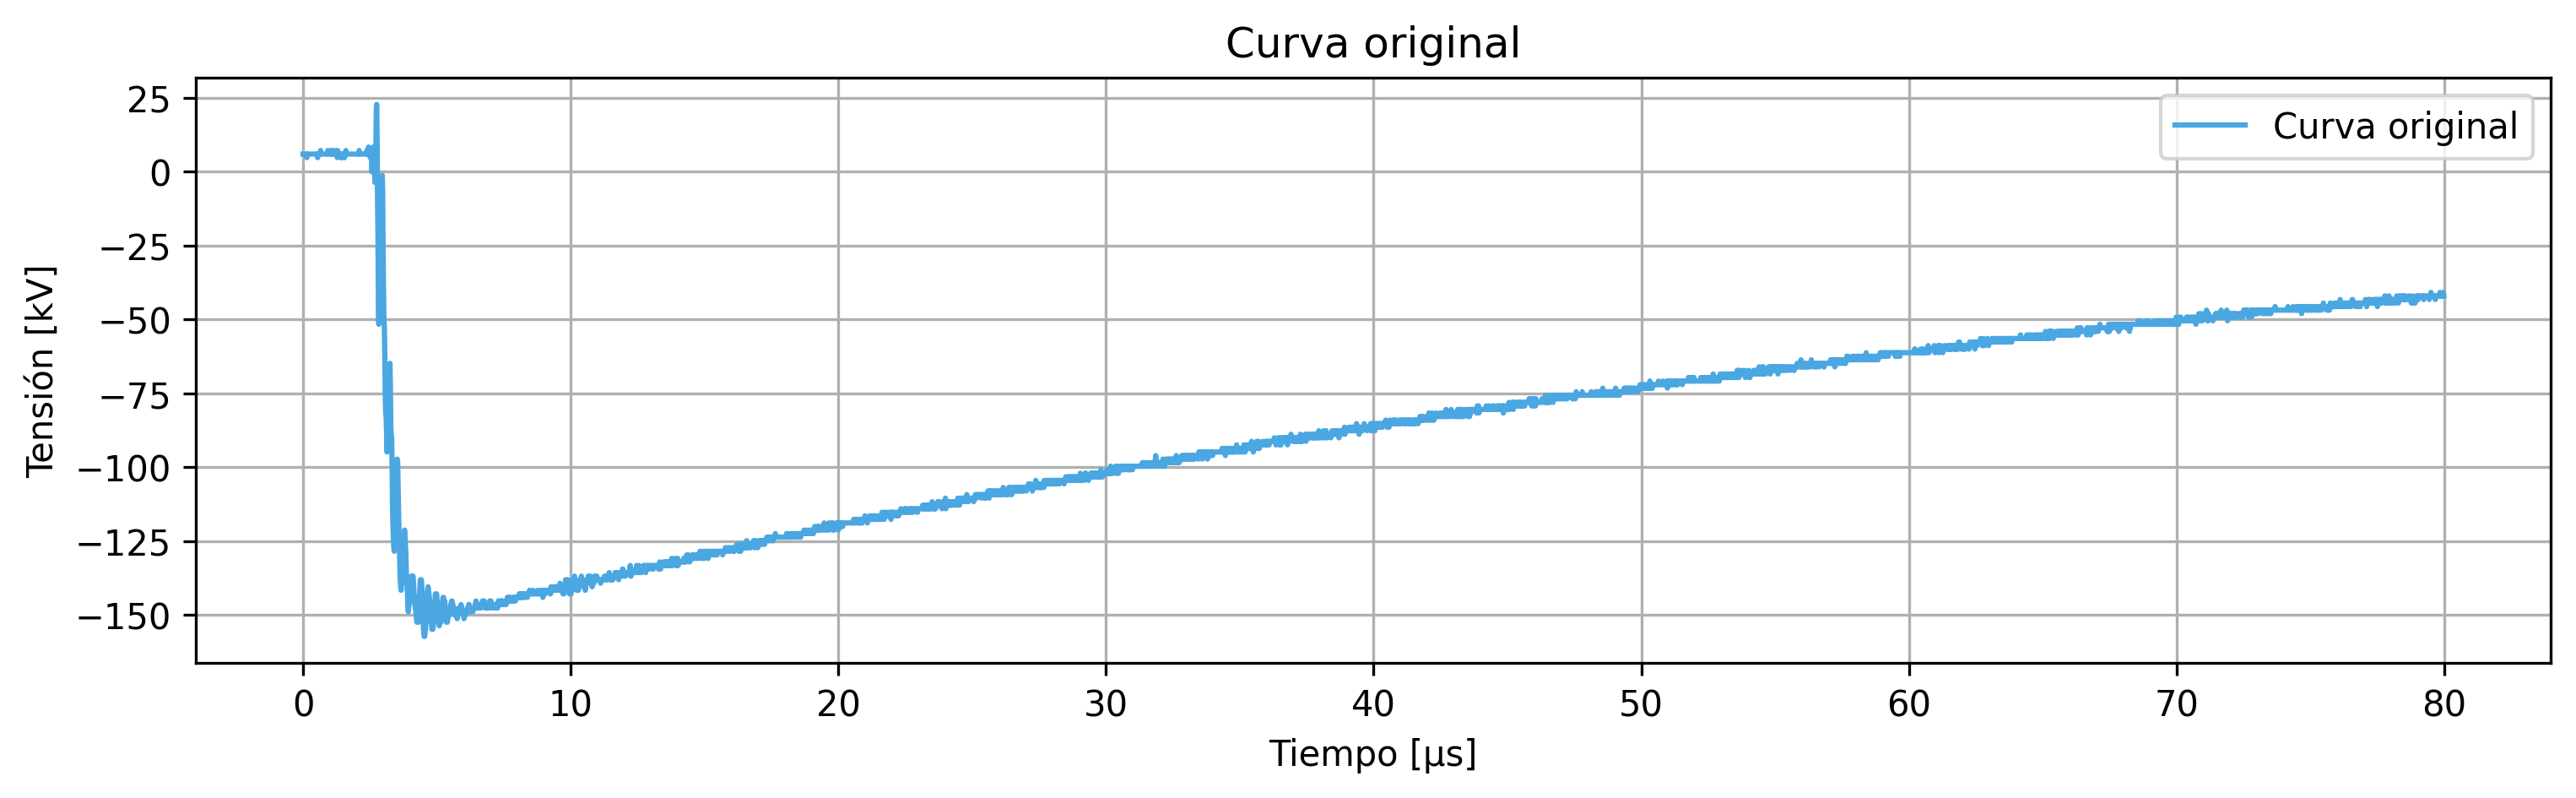
\includegraphics[width=\textwidth]{img/analisis_secuencial/LI/1_curva_original.png}
    \caption{Adquisición de datos: Señal discreta bruta $U_{e}[n]$ adquirida por el instrumento, presentando ruido electromagnético de alta frecuencia y nivel de continua previo al disparo.}
    \label{fig:curva_original}
\end{figure}
\vspace{3\baselineskip}

\vspace{3\baselineskip}
\begin{figure}[H]
    \centering
    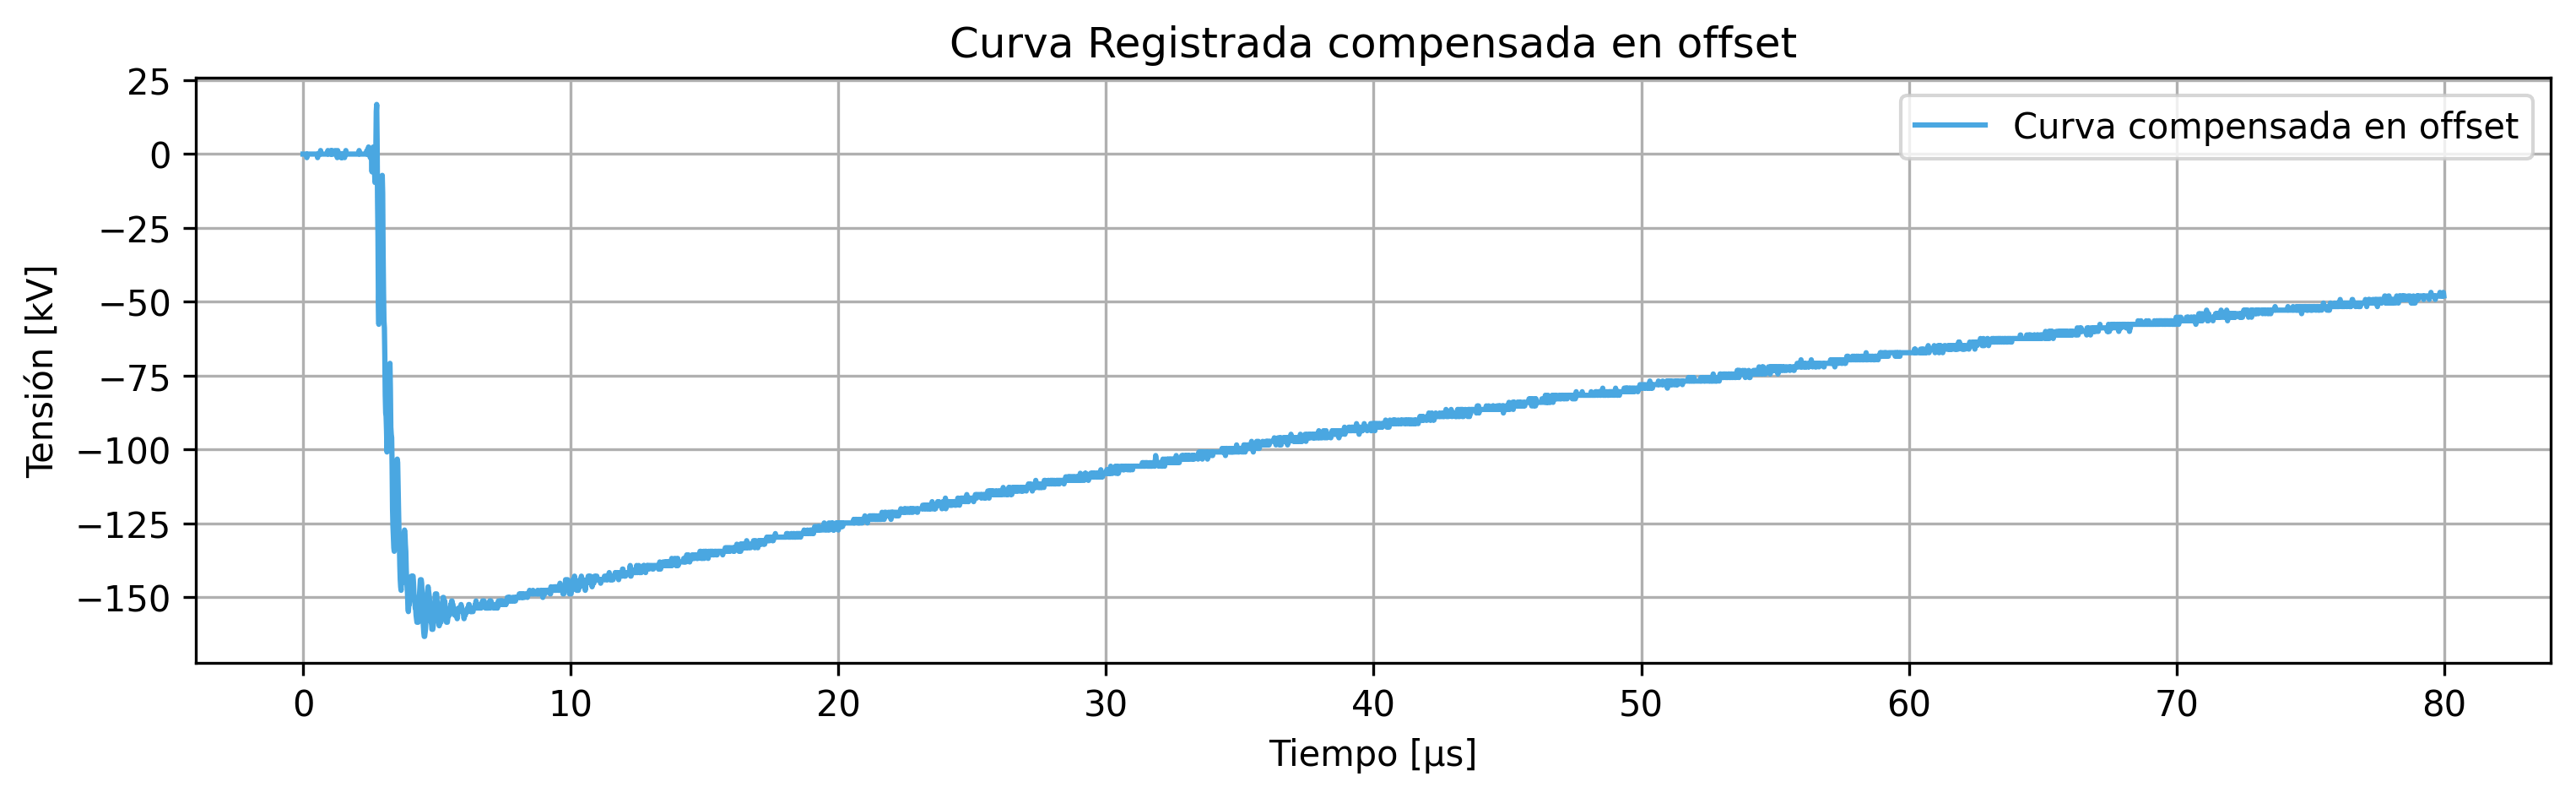
\includegraphics[width=\textwidth]{img/analisis_secuencial/LI/2_curva_compensada_offset.png}
    \caption{Fase I (Acondicionamiento): Curva resultante tras la sustracción del nivel de continua $V_{offset}$ calculado a partir de las muestras pre-disparo.}
    \label{fig:curva_offset}
\end{figure}
\vspace{3\baselineskip}

\vspace{3\baselineskip}
\begin{figure}[H]
    \centering
    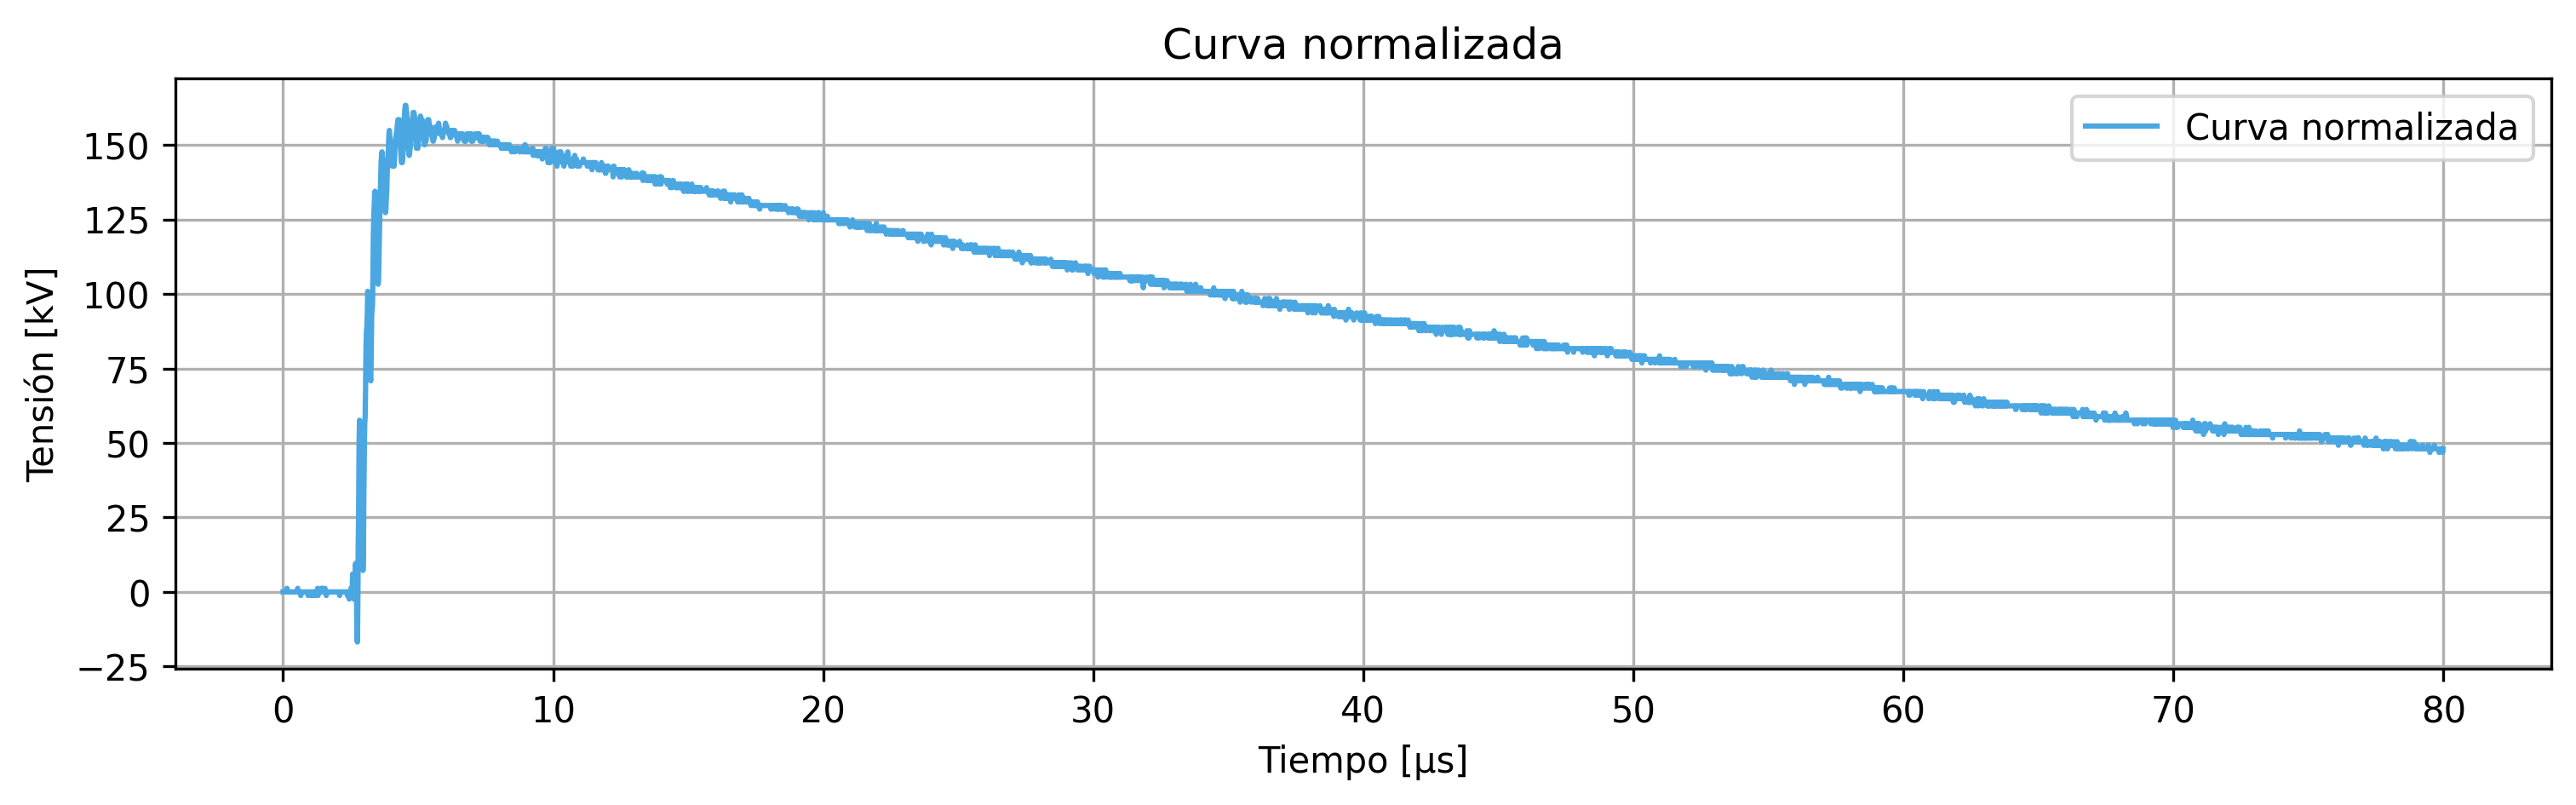
\includegraphics[width=\textwidth]{img/analisis_secuencial/LI/3_curva_positiva.png}
    \caption{Fase I (Normalización): Curva con polaridad normalizada hacia el semiplano positivo.}
    \label{fig:curva_positiva}
\end{figure}
\vspace{3\baselineskip}

\vspace{3\baselineskip}
\begin{figure}[H]
    \centering
    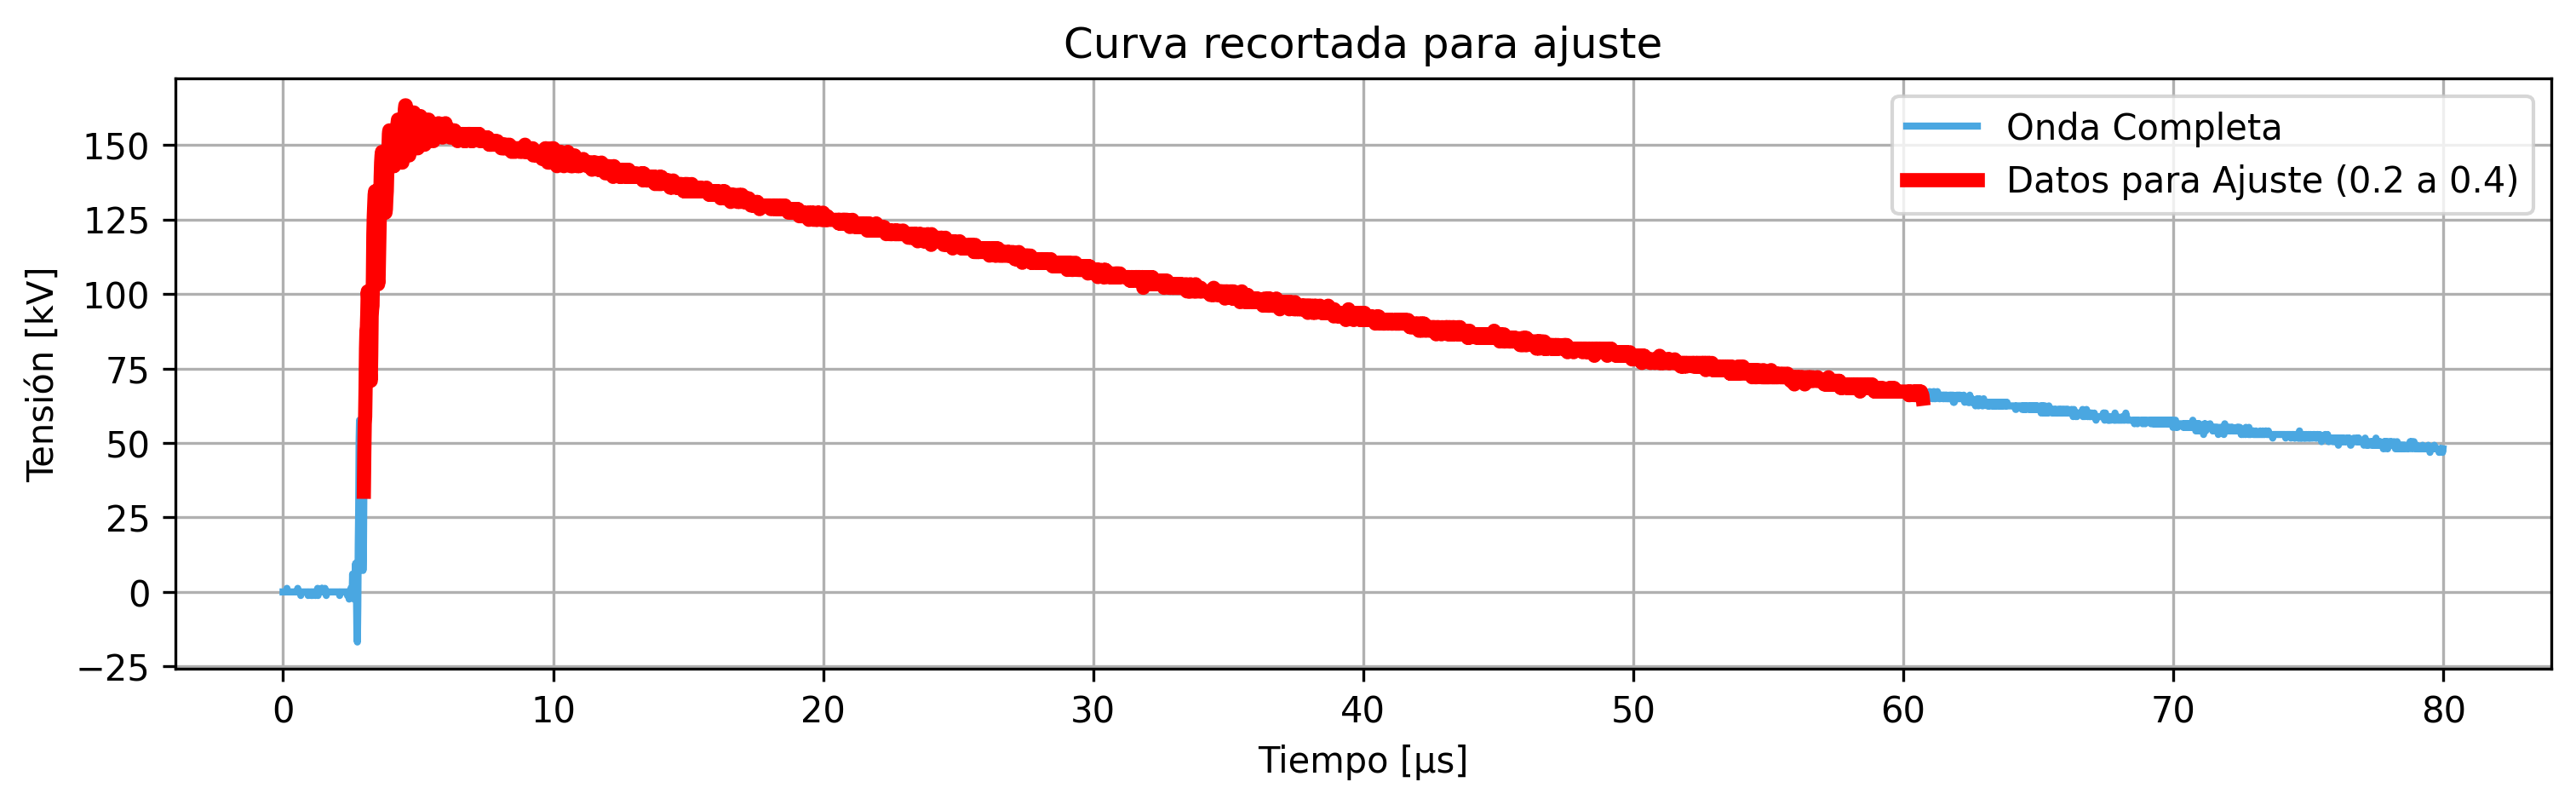
\includegraphics[width=\textwidth]{img/analisis_secuencial/LI/4_curva_recortada.png}
    \caption{Fase II (Segmentación): Delimitación de la ventana de datos útil (comprendida entre el \qty{20}{\percent} del frente y el \qty{40}{\percent} de la cola) para la regresión no lineal con el algoritmo de Levenberg-Marquardt~\cite{Chapra2015}.}
    \label{fig:curva_recortada}
\end{figure}
\vspace{3\baselineskip}

\vspace{3\baselineskip}
\begin{figure}[H]
    \centering
    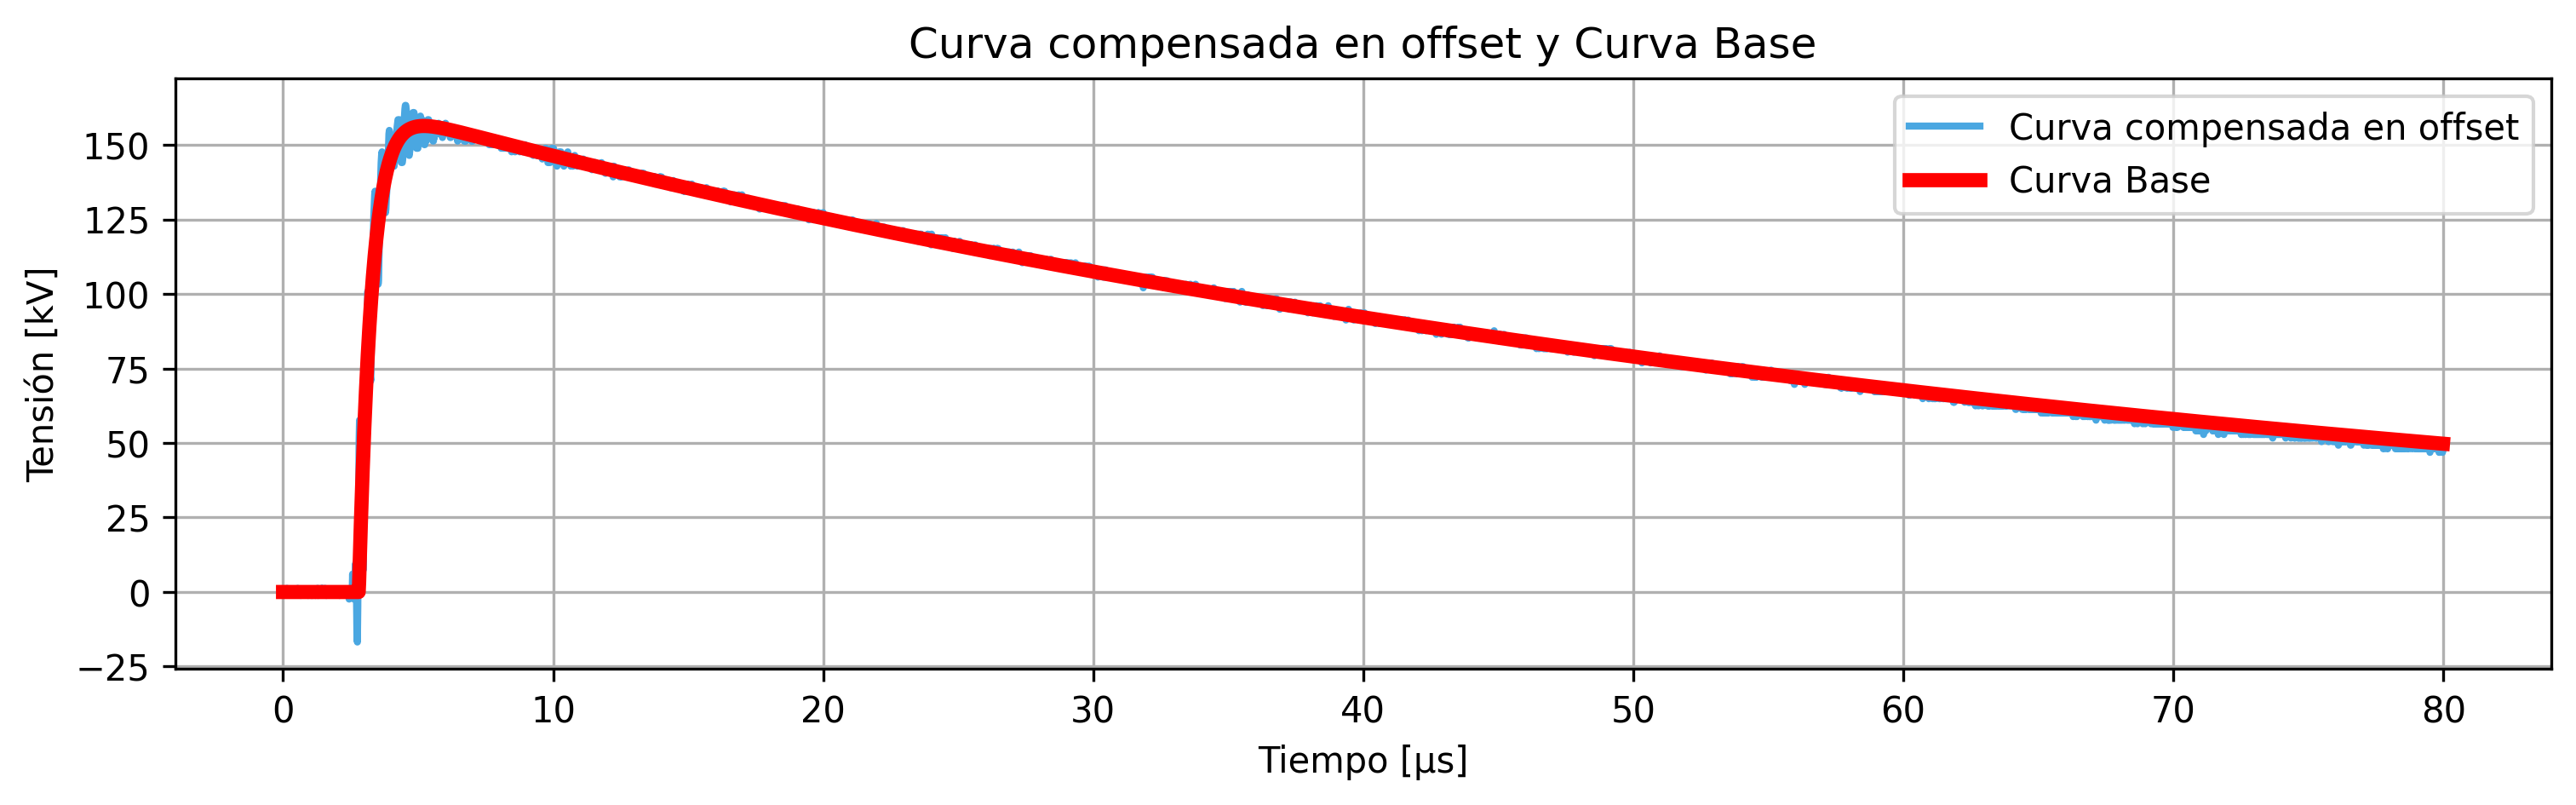
\includegraphics[width=\textwidth]{img/analisis_secuencial/LI/5_curva_base.png}
    \caption{Fase II (Ajuste de curva): Curva base $U_{b}[n]$ sintetizada sobre una función doble exponencial (ecuación \ref{eq:doble_exponencial}), superpuesta a la señal registrada.}
    \label{fig:curva_base}
\end{figure}
\vspace{3\baselineskip}

\vspace{3\baselineskip}
\begin{figure}[H]
    \centering
    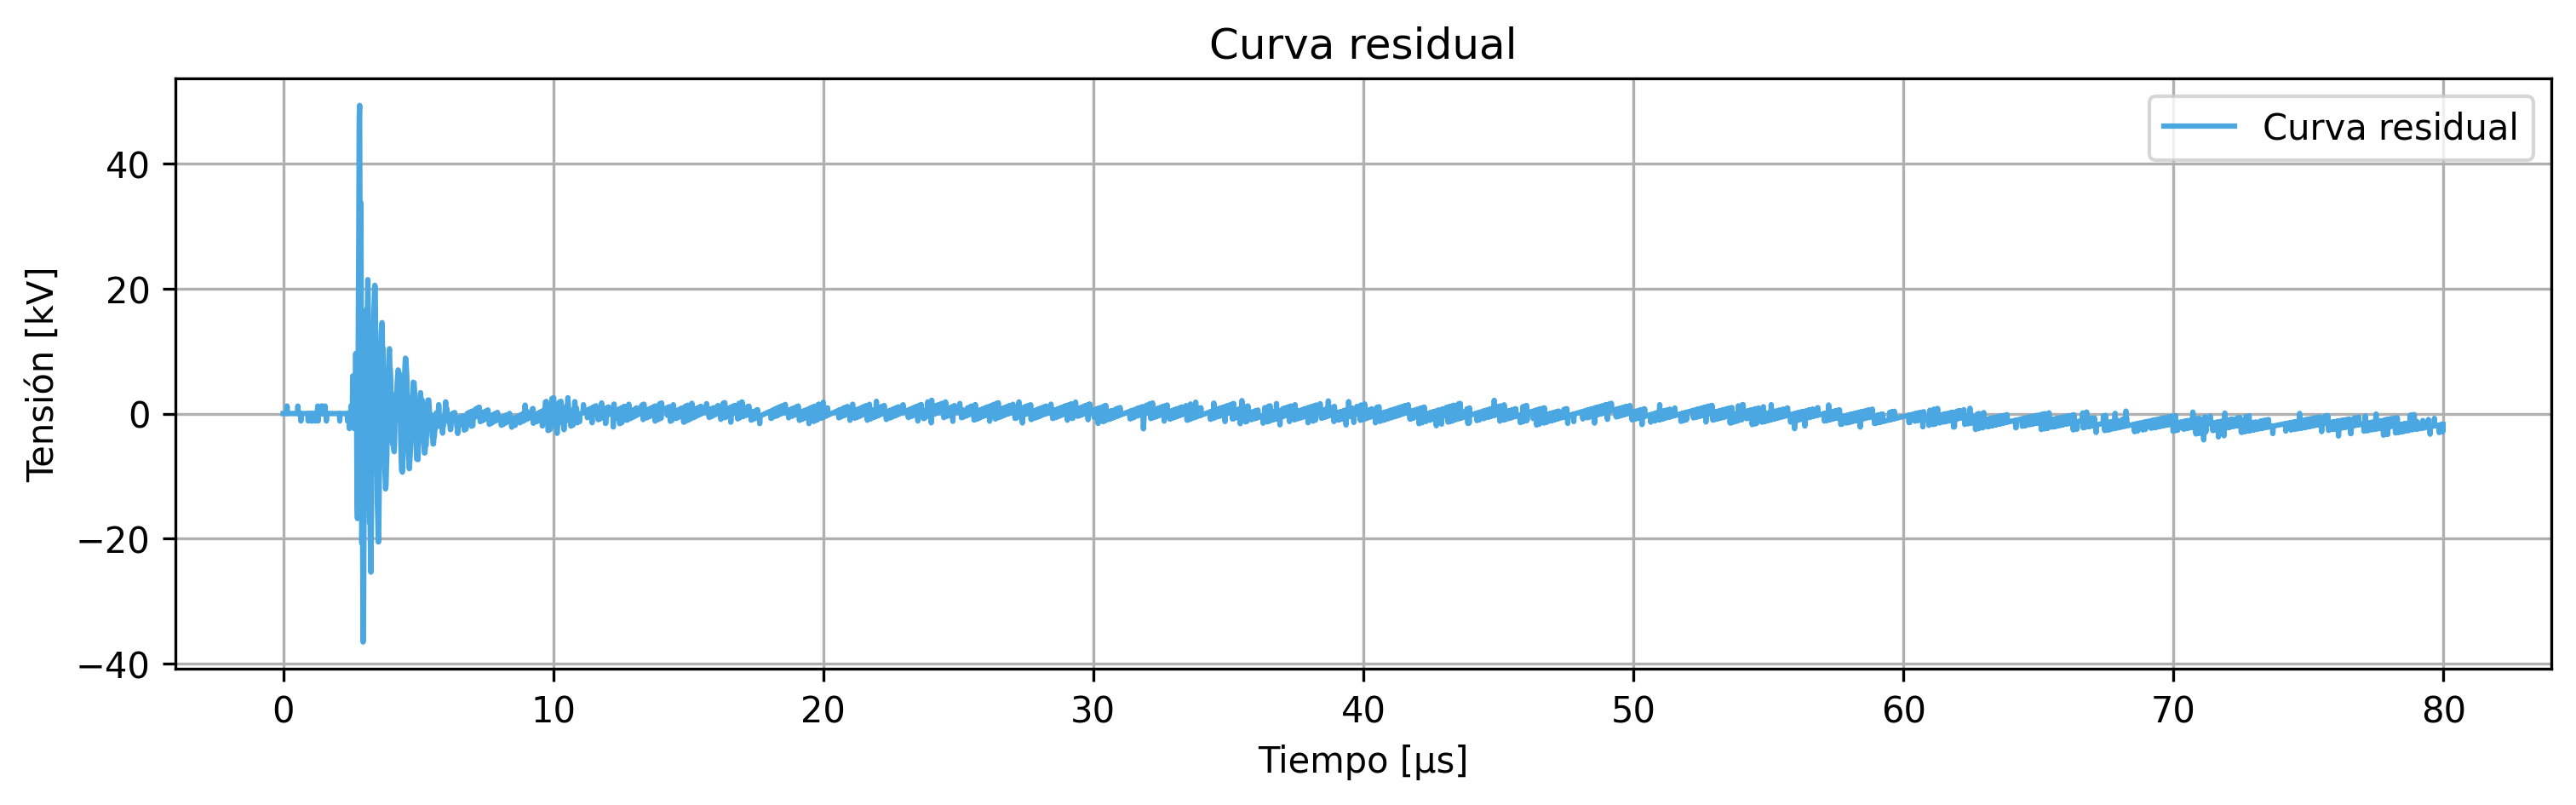
\includegraphics[width=\textwidth]{img/analisis_secuencial/LI/6_curva_residual.png}
    \caption{Fase III (Convergencia): Curva residual $R[n]$ obtenida por la diferencia algebraica entre la señal registrada y la curva base (ecuación \ref{eq:curva_residual}), aislando las oscilaciones y el ruido.}
    \label{fig:curva_residual}
\end{figure}
\vspace{3\baselineskip}

\vspace{3\baselineskip}
\begin{figure}[H]
    \centering
    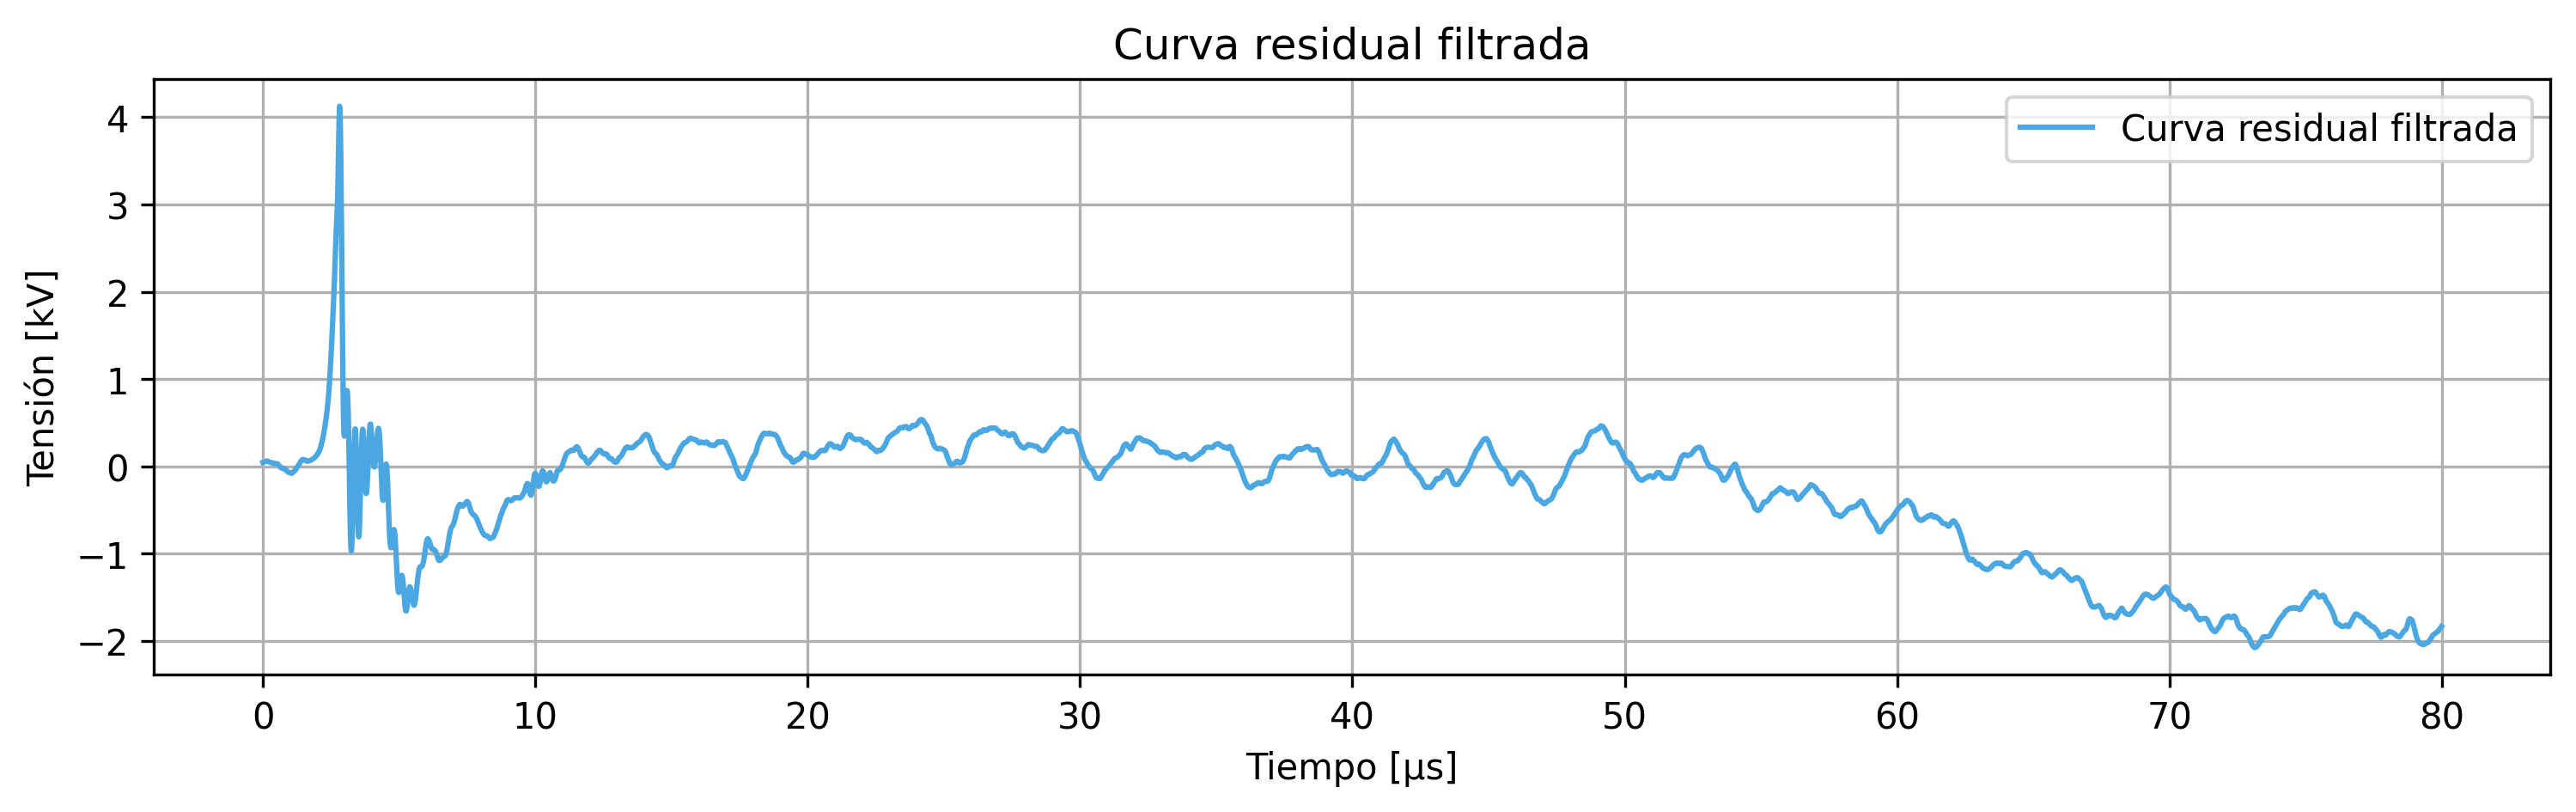
\includegraphics[width=\textwidth]{img/analisis_secuencial/LI/7_curva_residual_filtrada.png}
    \caption{Fase III (Filtrado): Curva residual filtrada $R_{f}[n]$ tras aplicar el filtro digital IIR de fase cero bidireccional (con la característica de la ecuación \ref{fig:funcion_tension_ensayo}), que mitiga la distorsión morfológica.}
    \label{fig:curva_filtrada}
\end{figure}
\vspace{3\baselineskip}

\vspace{3\baselineskip}
\begin{figure}[H]
    \centering
    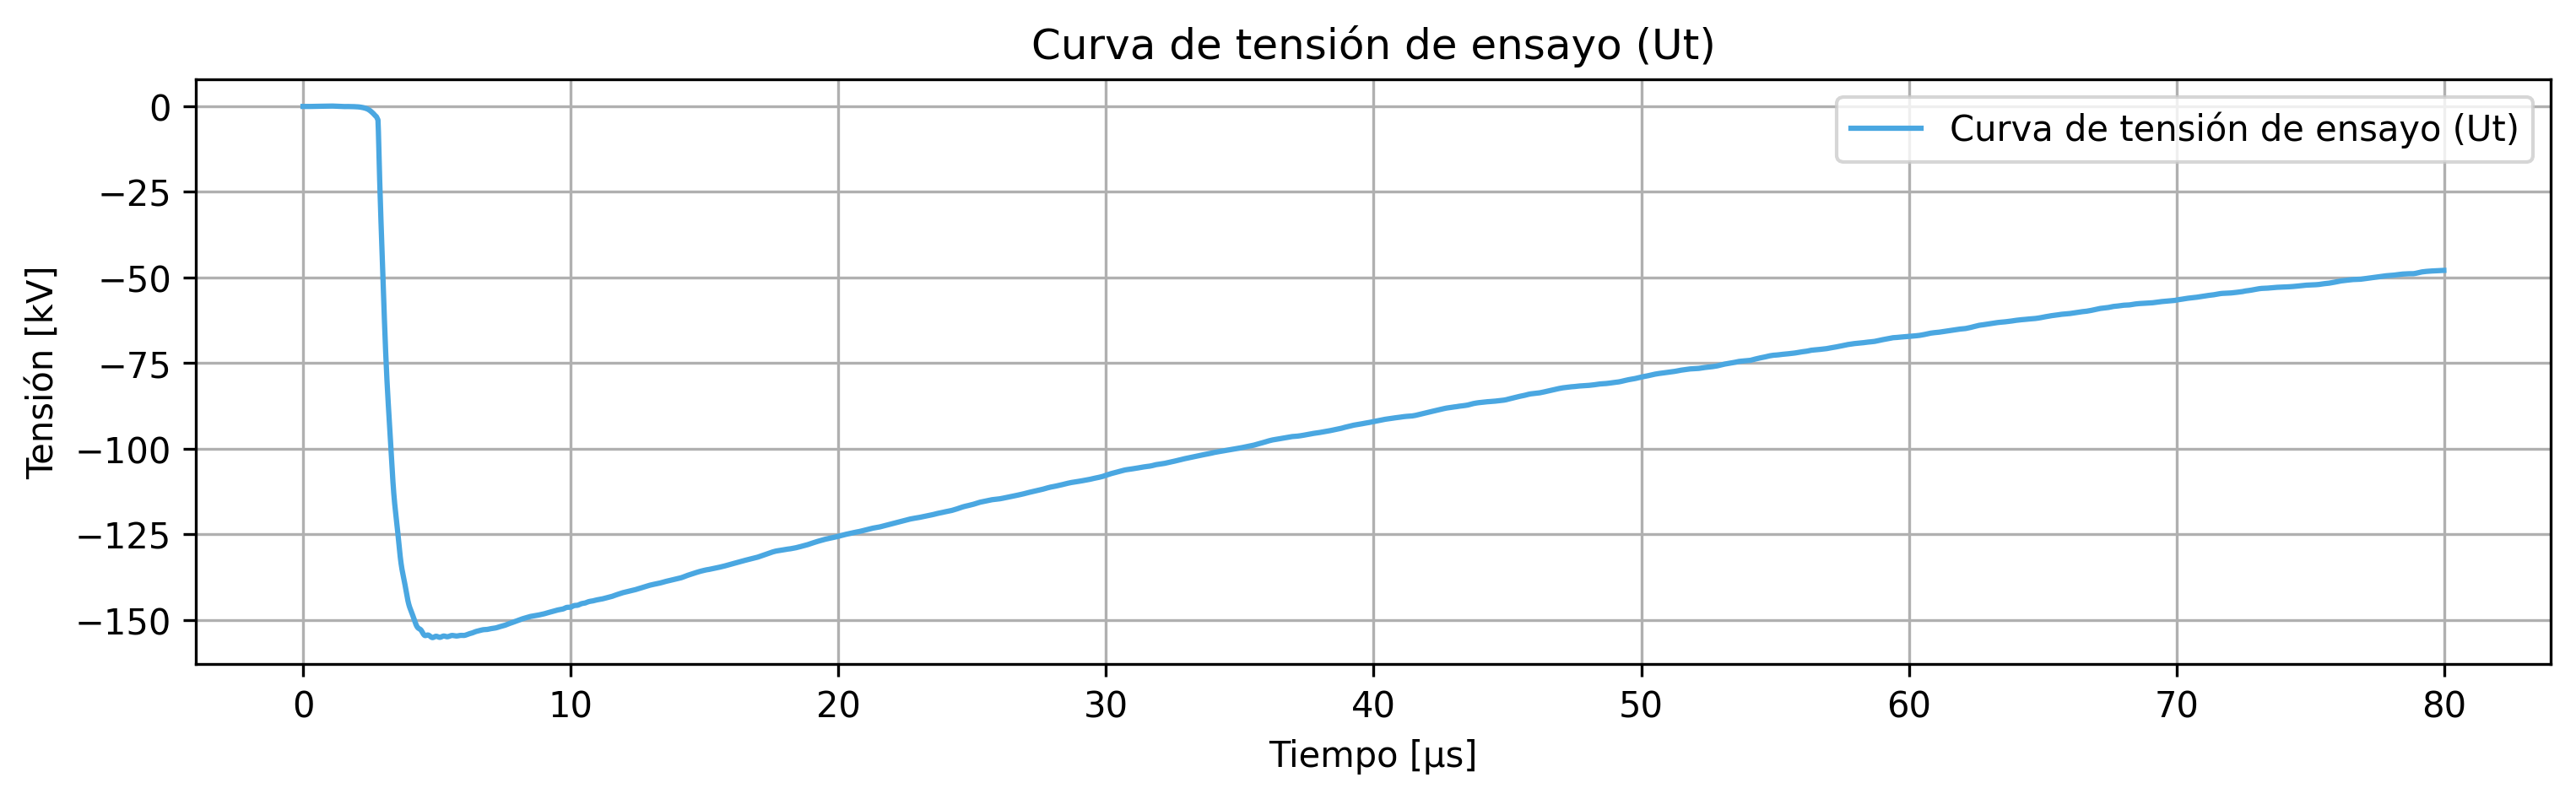
\includegraphics[width=\textwidth]{img/analisis_secuencial/LI/8_curva_ensayo.png}
    \caption{Fase III (Síntesis): Curva de tensión de ensayo $U_{t}[n]$, producto de la sumatoria entre la curva base y la curva residual filtrada (ecuación \ref{eq:curva_ensayo}).}
    \label{fig:curva_ensayo}
\end{figure}
\vspace{3\baselineskip}

\vspace{3\baselineskip}
\begin{figure}[H]
    \centering
    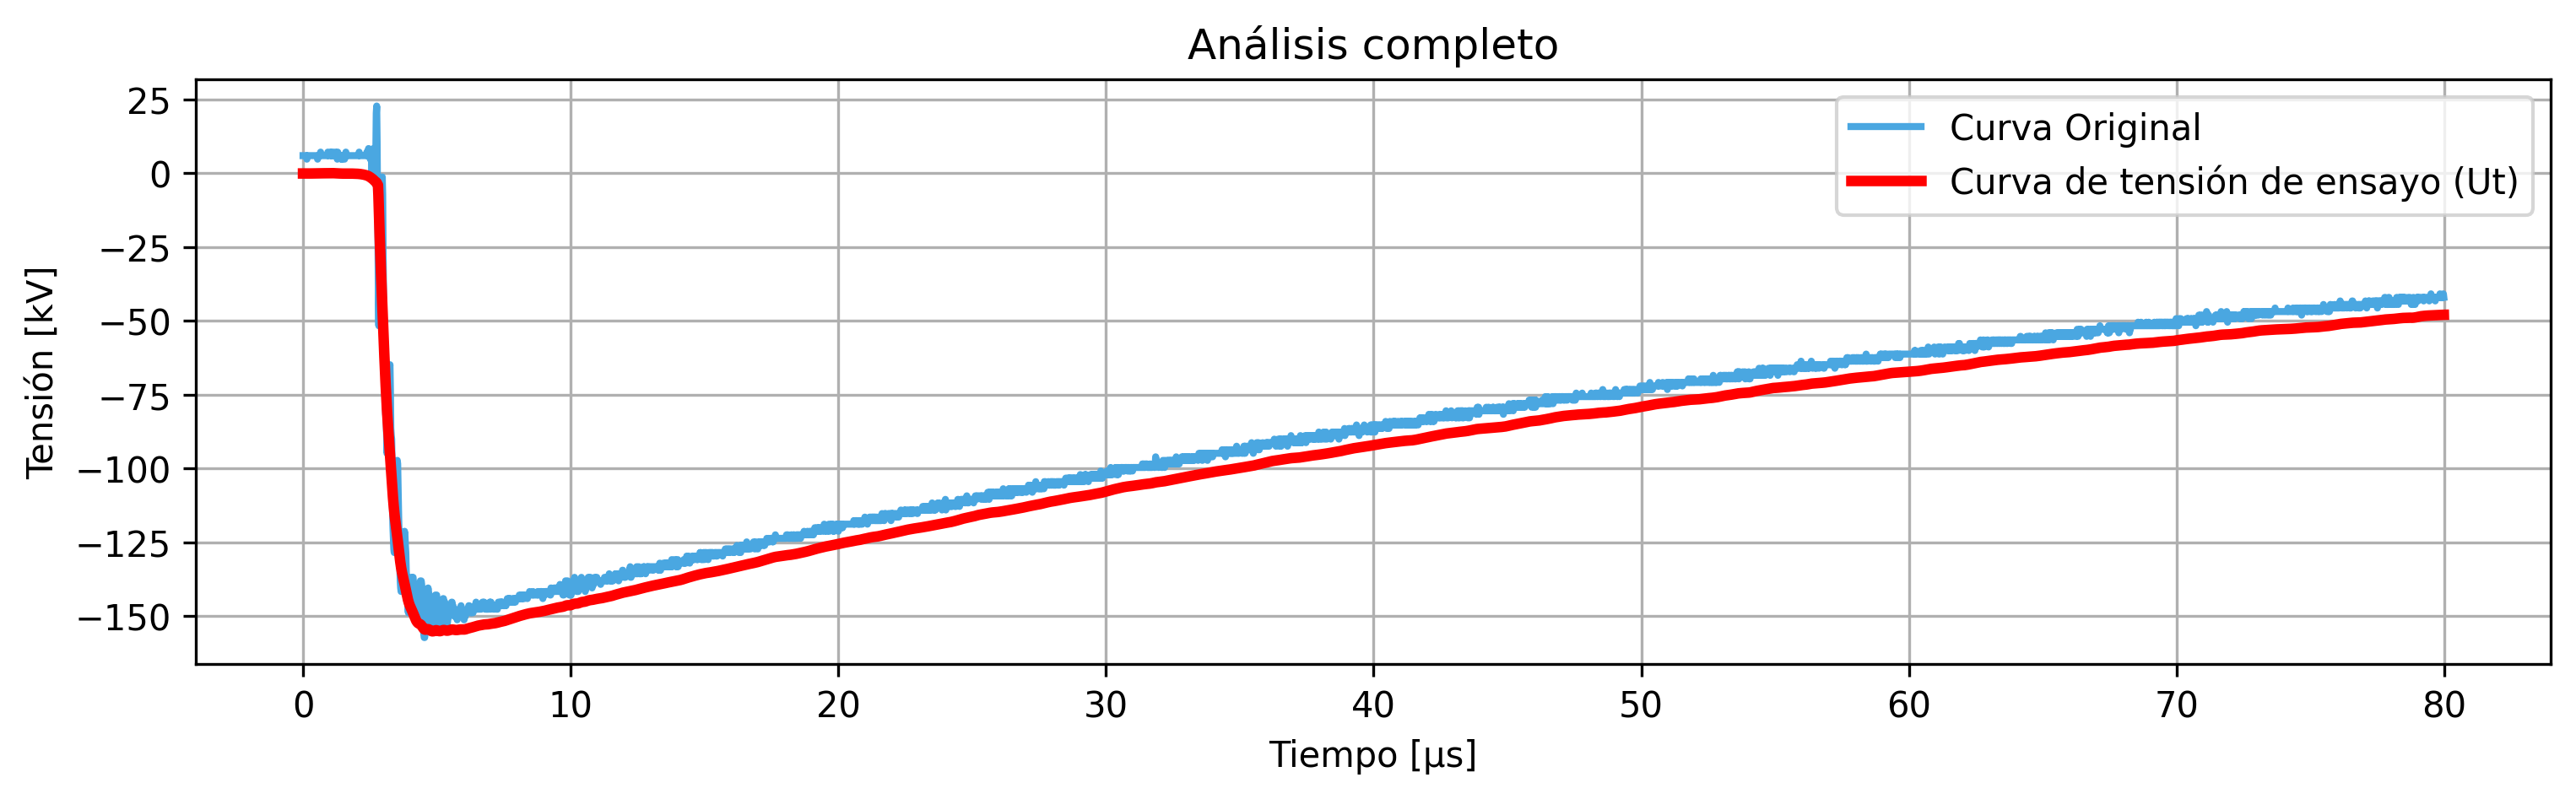
\includegraphics[width=\textwidth]{img/analisis_secuencial/LI/9_curva_original_ensayo.png}
    \caption{Resultado Final: Comparativa superpuesta entre la curva de tensión de ensayo procesada frente a la señal original bruta, evidenciando la eliminación de perturbaciones, lista para la extracción de sus parámetros $U_\text{t}$, $T_{1}$, $T_{2}$ y OS\%.}
    \label{fig:curva_final}
\end{figure}
\vspace{3\baselineskip}